% Options for packages loaded elsewhere
\PassOptionsToPackage{unicode}{hyperref}
\PassOptionsToPackage{hyphens}{url}
%
\documentclass[
  ignorenonframetext,
  aspectratio=43,
]{beamer}
\usepackage{pgfpages}
\setbeamertemplate{caption}[numbered]
\setbeamertemplate{caption label separator}{: }
\setbeamercolor{caption name}{fg=normal text.fg}
\beamertemplatenavigationsymbolshorizontal
% Prevent slide breaks in the middle of a paragraph
\widowpenalties 1 10000
\raggedbottom
\setbeamertemplate{part page}{
  \centering
  \begin{beamercolorbox}[sep=16pt,center]{part title}
    \usebeamerfont{part title}\insertpart\par
  \end{beamercolorbox}
}
\setbeamertemplate{section page}{
  \centering
  \begin{beamercolorbox}[sep=12pt,center]{part title}
    \usebeamerfont{section title}\insertsection\par
  \end{beamercolorbox}
}
\setbeamertemplate{subsection page}{
  \centering
  \begin{beamercolorbox}[sep=8pt,center]{part title}
    \usebeamerfont{subsection title}\insertsubsection\par
  \end{beamercolorbox}
}
\AtBeginPart{
  \frame{\partpage}
}
\AtBeginSection{
  \ifbibliography
  \else
    \frame{\sectionpage}
  \fi
}
\AtBeginSubsection{
  \frame{\subsectionpage}
}

\usepackage{amsmath,amssymb}
\usepackage{lmodern}
\usepackage{iftex}
\ifPDFTeX
  \usepackage[T1]{fontenc}
  \usepackage[utf8]{inputenc}
  \usepackage{textcomp} % provide euro and other symbols
\else % if luatex or xetex
  \usepackage{unicode-math}
  \defaultfontfeatures{Scale=MatchLowercase}
  \defaultfontfeatures[\rmfamily]{Ligatures=TeX,Scale=1}
\fi
\usetheme[]{default}
\usecolortheme{default}
% Use upquote if available, for straight quotes in verbatim environments
\IfFileExists{upquote.sty}{\usepackage{upquote}}{}
\IfFileExists{microtype.sty}{% use microtype if available
  \usepackage[]{microtype}
  \UseMicrotypeSet[protrusion]{basicmath} % disable protrusion for tt fonts
}{}
\makeatletter
\@ifundefined{KOMAClassName}{% if non-KOMA class
  \IfFileExists{parskip.sty}{%
    \usepackage{parskip}
  }{% else
    \setlength{\parindent}{0pt}
    \setlength{\parskip}{6pt plus 2pt minus 1pt}}
}{% if KOMA class
  \KOMAoptions{parskip=half}}
\makeatother
\usepackage{xcolor}
\newif\ifbibliography
\setlength{\emergencystretch}{3em} % prevent overfull lines
\setcounter{secnumdepth}{-\maxdimen} % remove section numbering


\providecommand{\tightlist}{%
  \setlength{\itemsep}{0pt}\setlength{\parskip}{0pt}}\usepackage{longtable,booktabs,array}
\usepackage{calc} % for calculating minipage widths
\usepackage{caption}
% Make caption package work with longtable
\makeatletter
\def\fnum@table{\tablename~\thetable}
\makeatother
\usepackage{graphicx}
\makeatletter
\def\maxwidth{\ifdim\Gin@nat@width>\linewidth\linewidth\else\Gin@nat@width\fi}
\def\maxheight{\ifdim\Gin@nat@height>\textheight\textheight\else\Gin@nat@height\fi}
\makeatother
% Scale images if necessary, so that they will not overflow the page
% margins by default, and it is still possible to overwrite the defaults
% using explicit options in \includegraphics[width, height, ...]{}
\setkeys{Gin}{width=\maxwidth,height=\maxheight,keepaspectratio}
% Set default figure placement to htbp
\makeatletter
\def\fps@figure{htbp}
\makeatother

\usepackage{ragged2e}
\usepackage{etoolbox}

\apptocmd{\frame}{}{\justifying}{} 

\setbeamertemplate{enumerate items}[default]
\setbeamertemplate{itemize items}[circle]
\setbeamersize{text margin left=2.25em, text margin right=2.25em}

\let\OLDitemize\itemize
\renewcommand\itemize{
    \OLDitemize\addtolength{\itemsep}{3pt plus 1pt minus 1pt}
}
\let\OLDenumerate\enumerate
\renewcommand\enumerate{
    \OLDenumerate\addtolength{\itemsep}{3pt plus 1pt minus 1pt}
}

\usepackage{orcidlink}
\usepackage{amsmath}
\DeclareMathOperator*{\argmax}{argmax}

\makeatletter
\def\@listii{\leftmargin\leftmarginii
              \topsep    1ex
              \parsep    0\p@   \@plus\p@
              \itemsep   \parsep}
\makeatother

\usepackage{lipsum}

\let\olditem\item
\renewcommand\item{\olditem\justifying}

\definecolor{blue}{RGB}{0,114,178}
\definecolor{red}{RGB}{213,94,0}
\definecolor{yellow}{RGB}{240,228,66}
\definecolor{green}{RGB}{0,158,115}

\definecolor{MyBackground}{RGB}{255,253,218}

\setbeamercolor{section in toc}{fg=blue}
\setbeamercolor{subsection in toc}{fg=red}

\setbeamercolor{frametitle}{fg=blue}
\setbeamercolor{title}{fg=blue}

\setbeamertemplate{footline}[frame number]
\setbeamertemplate{navigation symbols}{} 
\setbeamertemplate{itemize items}{-}

\setbeamercolor{itemize item}{fg=blue}
\setbeamercolor{itemize subitem}{fg=blue}
\setbeamercolor{enumerate item}{fg=blue}
\setbeamercolor{enumerate subitem}{fg=blue}
\setbeamercolor{button}{bg=MyBackground,fg=blue}

\newcounter{daggerfootnote}
\newcommand*{\daggerfootnote}[1]{%
    \setcounter{daggerfootnote}{\value{footnote}}%
    \renewcommand*{\thefootnote}{\fnsymbol{footnote}}%
    \footnote[2]{#1}%
    \setcounter{footnote}{\value{daggerfootnote}}%
    \renewcommand*{\thefootnote}{\arabic{footnote}}%
}

\AtBeginSection{
    \begingroup
    \setbeamercolor{background canvas}{bg=yellow}
    \begin{frame}
        \begin{centering}
            \usebeamerfont{section title}\huge\color{black}\insertsection\par
        \end{centering}
    \end{frame}
    \endgroup
}
\makeatletter
\makeatother
\makeatletter
\makeatother
\makeatletter
\@ifpackageloaded{caption}{}{\usepackage{caption}}
\AtBeginDocument{%
\ifdefined\contentsname
  \renewcommand*\contentsname{Table of contents}
\else
  \newcommand\contentsname{Table of contents}
\fi
\ifdefined\listfigurename
  \renewcommand*\listfigurename{List of Figures}
\else
  \newcommand\listfigurename{List of Figures}
\fi
\ifdefined\listtablename
  \renewcommand*\listtablename{List of Tables}
\else
  \newcommand\listtablename{List of Tables}
\fi
\ifdefined\figurename
  \renewcommand*\figurename{Figure}
\else
  \newcommand\figurename{Figure}
\fi
\ifdefined\tablename
  \renewcommand*\tablename{Table}
\else
  \newcommand\tablename{Table}
\fi
}
\@ifpackageloaded{float}{}{\usepackage{float}}
\floatstyle{ruled}
\@ifundefined{c@chapter}{\newfloat{codelisting}{h}{lop}}{\newfloat{codelisting}{h}{lop}[chapter]}
\floatname{codelisting}{Listing}
\newcommand*\listoflistings{\listof{codelisting}{List of Listings}}
\makeatother
\makeatletter
\@ifpackageloaded{caption}{}{\usepackage{caption}}
\@ifpackageloaded{subcaption}{}{\usepackage{subcaption}}
\makeatother
\makeatletter
\@ifpackageloaded{tcolorbox}{}{\usepackage[many]{tcolorbox}}
\makeatother
\makeatletter
\@ifundefined{shadecolor}{\definecolor{shadecolor}{rgb}{.97, .97, .97}}
\makeatother
\makeatletter
\makeatother
\ifLuaTeX
  \usepackage{selnolig}  % disable illegal ligatures
\fi
\IfFileExists{bookmark.sty}{\usepackage{bookmark}}{\usepackage{hyperref}}
\IfFileExists{xurl.sty}{\usepackage{xurl}}{} % add URL line breaks if available
\urlstyle{same} % disable monospaced font for URLs
\hypersetup{
  pdftitle={Seminar 1},
  pdfauthor={Gabriel E. Cabrera Guzmán},
  hidelinks,
  pdfcreator={LaTeX via pandoc}}

\title[Seminar 1]{Seminar
1\daggerfootnote{\texttt{gabriel.cabreraguzman@postgrad.manchester.ac.uk}}}
\subtitle{Describing Data 1 (Data Visualization)}
\author[Gabriel E. Cabrera Guzmán]{
    {Gabriel E. Cabrera
Guzmán\textsuperscript{\normalsize\orcidlink{0000-0000-0000-0000}}} \medskip
}
\date{October 9, 2025}
\institute[]{
    The University of Manchester\\
Alliance Manchester Business School \bigskip
}

\definecolor{quarto-callout-note-color}{RGB}{0,114,178}
\definecolor{quarto-callout-note-color-frame}{RGB}{0,114,178}
\definecolor{quarto-callout-warning-color}{RGB}{213,94,0}
\definecolor{quarto-callout-warning-color-frame}{RGB}{213,94,0}
\begin{document}
\frame{\titlepage}
\ifdefined\Shaded\renewenvironment{Shaded}{\begin{tcolorbox}[boxrule=0pt, frame hidden, borderline west={3pt}{0pt}{shadecolor}, interior hidden, enhanced, sharp corners, breakable]}{\end{tcolorbox}}\fi

\begin{frame}{Exercise 1}
\protect\hypertarget{exercise-1}{}
What sort of display would be most suitable for the following data?

\begin{enumerate}
\item
  The \textbf{amount of taxation} paid by a light engineering company
  and \textbf{its annual profit} for \textbf{20 consecutive years.}

  \pause

  \textbf{A:} This is a comparison between 2 numerical measures. Hence,
  a scatter plot would be the most suitable.

  \pause
\item
  The \textbf{types} of premises occupied by all the small businesses in
  a town -- \textbf{office, factory, warehouse,} etc.

  \pause

  \textbf{A:} These are categorical variables. Hence, Bar Chart or Pie
  Chart would be the most suitable visualisation.
\end{enumerate}
\end{frame}

\begin{frame}{Exercise 1 (Cont'd)}
\protect\hypertarget{exercise-1-contd}{}
\begin{enumerate}
\setcounter{enumi}{2}
\item
  The \textbf{salary} of a trainee accountant in his/her first year of
  training at 30 major accountancy firms.

  \pause

  \textbf{A:} There is one numerical measure (salaries). Hence,
  Histogram or Stem \& Leaf would be the most suitable visualisation.

  \pause
\item
  The \textbf{number of trainee accountants} enrolling for professional
  examinations \textbf{each year since 1960}.

  \pause

  \textbf{A:} Although there is only one numerical measure, but it must
  be illustrated with respect to time. Therefore, Time Series Plot would
  be most suitable.
\end{enumerate}
\end{frame}

\begin{frame}{Exercise 1 (Cont'd)}
\protect\hypertarget{exercise-1-contd-1}{}
\begin{enumerate}
\setcounter{enumi}{4}
\item
  The \textbf{number of years of experience} and \textbf{the current
  salary} of a random sample of economists working for a New York bank.

  \pause

  \textbf{A:} This is a comparison between 2 numerical measures. Hence,
  a scatter plot would be the most suitable.
\end{enumerate}
\end{frame}

\begin{frame}{Exercise 2}
\protect\hypertarget{exercise-2}{}
In one year, the executive pay, including salary and bonus, in millions
of dollars, for 28 chairpersons and chief executive officers are
presented in the table below. Display these data by drawing a histogram
using Excel. \vspace{10pt}

\begin{table}
\centering
\tiny
\resizebox{0.8\textwidth}{!}{
\begin{tabular}{lrlr}
\toprule
Company & Value & Company & Value \\
\midrule
Boeing & 21.12 & Coca-Cola & 21.60 \\
Whirlpool & 12.93 & DuPont & 12.73 \\
Bank of America & 12.00 & Motorola & 47.15 \\
Sherwin-Williams & 11.00 & Marriott & 8.58 \\
Bristol-Myers Squibb & 16.00 & Honeywell & 16.28 \\
General Mills & 12.19 & Exxon & 34.90 \\
Hillshire Brands & 6.40 & CBS & 60.25 \\
Wal-Mart & 20.70 & AT\&T & 21.00 \\
Apple & 4.17 & Philip Morris & 24.73 \\
Goodyear & 13.43 & Tesco & 1.90 \\
Teledyne & 3.21 & EasyJet & 6.40 \\
Delta Airlines & 12.58 & Shell & 5.10 \\
Chrysler & 1.23 & GlaxoSmithKline & 6.39 \\
\bottomrule
\end{tabular}
}
\end{table}
\end{frame}

\begin{frame}{Exercise 2 (Cont'd)}
\protect\hypertarget{exercise-2-contd}{}
\begin{figure}

{\centering 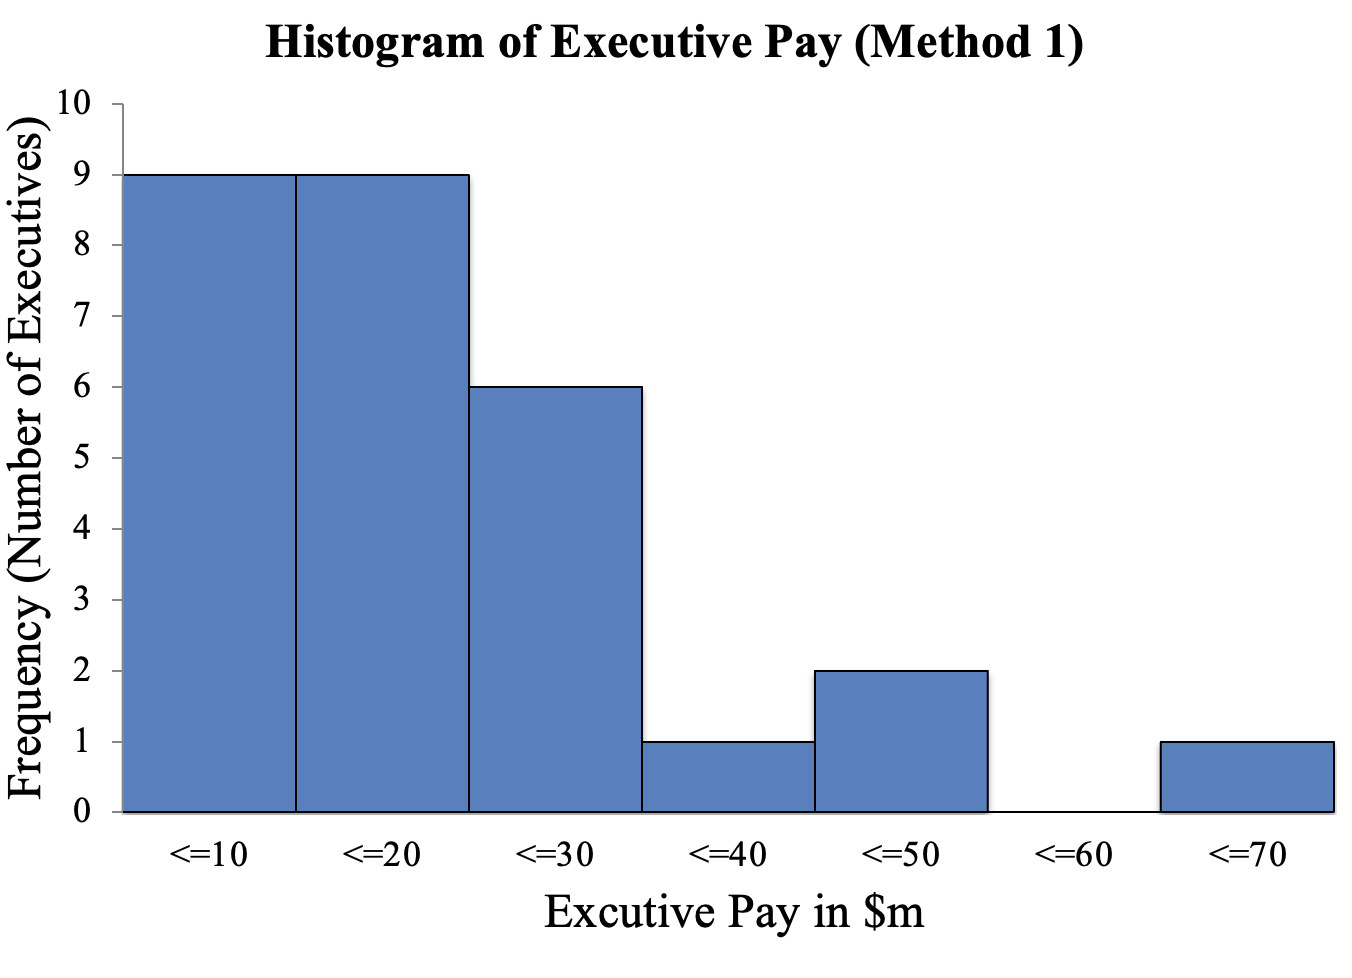
\includegraphics[width=0.85\textwidth,height=0.85\textheight]{Fig/q2_histogram.png}

}

\end{figure}
\end{frame}

\begin{frame}{Exercise 3}
\protect\hypertarget{exercise-3}{}
A financial analyst is interested in the amount of resources spent by
computer companies on Research and Development (R\&D). She samples 30
such firms and calculates the percentage of total revenue they spent on
R\&D in the last year. The results are given below. Summarize these data
using by using: a) the frequencies, b) the relative frequencies, c) a
histogram.

\begin{table}
\centering
\tiny
\resizebox{0.8\textwidth}{!}{
\begin{tabular}{llllll}
\toprule
Company & (\%) & Company & (\%) & Company & (\%) \\
\midrule
1  &  6.0 & 11 &  7.9 & 21 &  8.0 \\
2  & 10.4 & 12 &  6.8 & 22 &  7.7 \\
3  & 10.5 & 13 &  7.4 & 23 &  7.4 \\
4  &  9.0 & 14 &  9.5 & 24 &  6.5 \\
5  &  7.3 & 15 &  8.1 & 25 &  9.5 \\
6  &  6.6 & 16 & 13.5 & 26 &  8.2 \\
7  &  6.9 & 17 &  9.9 & 27 &  6.9 \\
8  &  8.2 & 18 &  6.9 & 28 &  7.2 \\
9  &  7.1 & 19 & 11.1 & 29 &  8.2 \\
10 &  8.1 & 20 &  8.2 & 30 &  6.7 \\
\bottomrule
\end{tabular}
}
\end{table}

Also, use the histogram to deduce the proportion of companies that spend
\textbf{more than 9\%} on R\&D.
\end{frame}

\begin{frame}{Exercise 3 (Cont'd)}
\protect\hypertarget{exercise-3-contd}{}
\textbf{A:} For a) and b) \vspace{10pt}

\begin{table}
\centering
\normalsize
\resizebox{0.65\textwidth}{!}{
\begin{tabular}{ccc}
\toprule
\textbf{Bin} & \textbf{Frequency} & \textbf{Relative Frequency} \\
\midrule
7  &  8 & 26.7\% \\
8  &  8 & 26.7\% \\
9  &  7 & 23.3\% \\
10 &  3 & 10.0\% \\
11 &  2 &  6.7\% \\
12 &  1 &  3.3\% \\
13 &  0 &  0.0\% \\
14 &  1 &  3.3\% \\
\midrule
\textbf{Total} & \textbf{30} & \textbf{100\%} \\
\bottomrule
\end{tabular}
}
\end{table}
\end{frame}

\begin{frame}{Exercise 3 (Cont'd)}
\protect\hypertarget{exercise-3-contd-1}{}
For c) \vspace{10pt}

\begin{figure}

{\centering 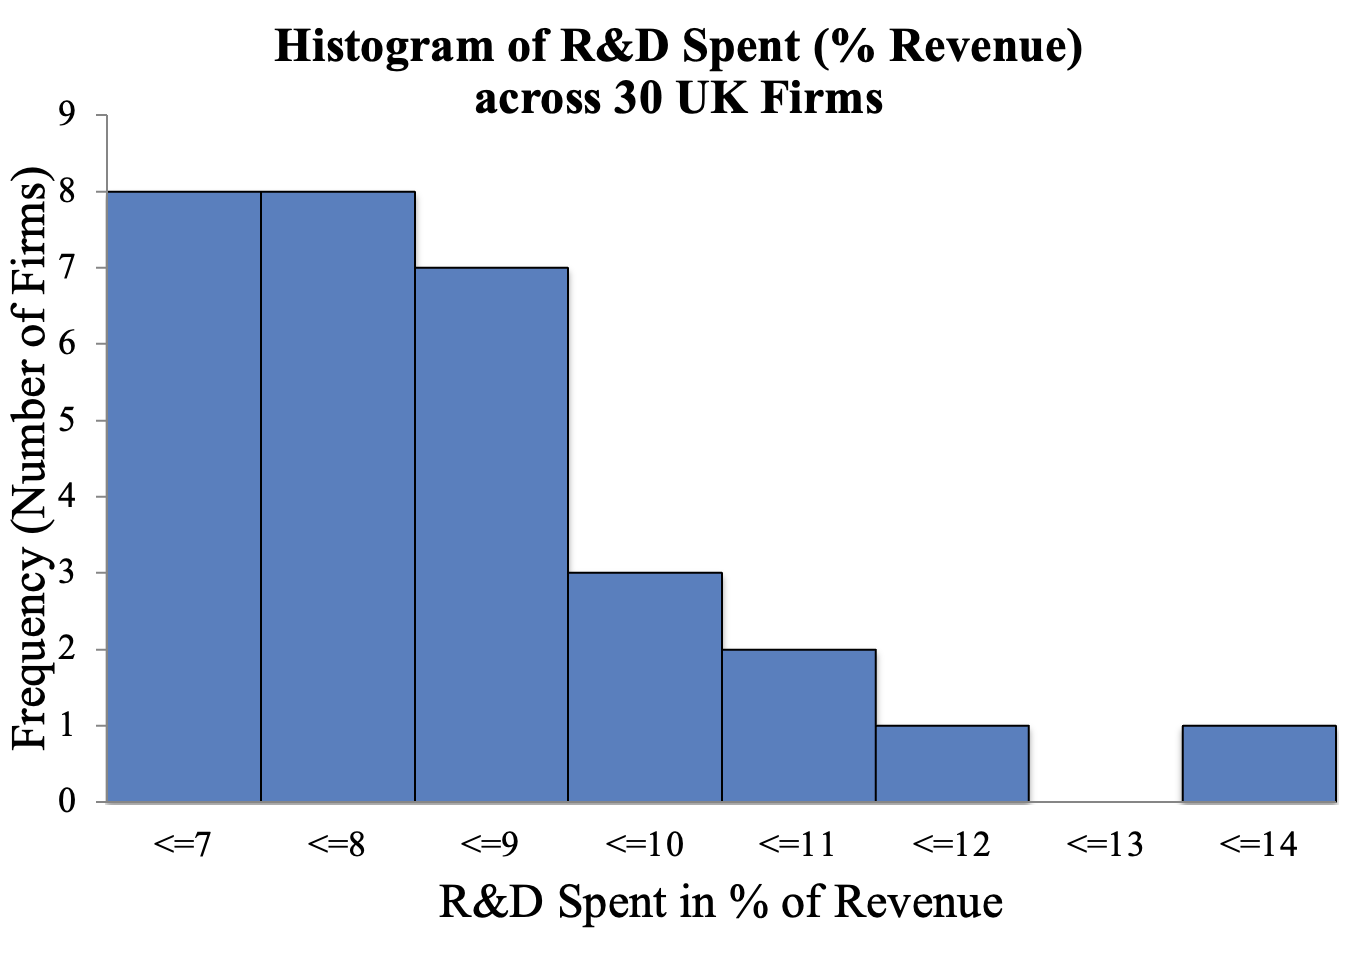
\includegraphics[width=0.75\textwidth,height=0.75\textheight]{Fig/q3_histogram.png}

}

\end{figure}

Therefore, 7/30 companies spend 9\% or more on R\&D.
\end{frame}

\begin{frame}{Exercise 4}
\protect\hypertarget{exercise-4}{}
Choosing a suitable leaf unit, draw a stem and leaf diagram \textbf{by
hand} for the list of executive salaries given below in thousands of
pounds. The data are: \vspace{10pt}

\begin{table}
\centering
\scriptsize
\resizebox{0.7\textwidth}{!}{
\begin{tabular}{ccccc}
\toprule
846 & 457 & 563 & 1466 & 1200 \\
2164 & 746 & 1611 & 824 & 824 \\
1310 & 1007 & 1367 & 575 & 1252 \\
1354 & 2479 & 1238 & 927 & 1253 \\
925 & 1284 & 1279 & 1660 & 860 \\
\bottomrule
\end{tabular}
}
\end{table}
\end{frame}

\begin{frame}{Exercise 4 (Cont'd)}
\protect\hypertarget{exercise-4-contd}{}
\textbf{A:} Taking a stem unit of 1000 and leaf unit of 100 gives only
three classes but allowing two rows for each stem unit overcomes this.
We have rounded to obtain the leaf unit. For example, the first data
point (846) can be approximated to 800, which is written in the form of
0 × 1000 + 8 × 100. This means that the number of stem is zero and there
are 8 leaves. Consider another example: 2164 is approximated to 2200 and
is written as 2 × 1000 + 2 × 100. Repeating this, the original data
becomes: \vspace{10pt}

\begin{table}
\centering
\tiny
\resizebox{0.7\textwidth}{!}{
\begin{tabular}{ccccc}
\toprule
800 & 500 & 600 & 1500 & 1200 \\
2200 & 700 & 1600 & 800 & 800 \\
1300 & 1000 & 1400 & 600 & 1300 \\
1400 & 2500 & 1200 & 900 & 1300 \\
900 & 1300 & 1300 & 1700 & 900 \\
\bottomrule
\end{tabular}
}
\end{table}
\end{frame}

\begin{frame}{Exercise 4 (Cont'd)}
\protect\hypertarget{exercise-4-contd-1}{}
\textbf{A:} The above data can be presented as follows: \vspace{10pt}

\begin{table}
\centering
\tiny
\resizebox{0.6\textwidth}{!}{
\begin{tabular}{cl}
\toprule
\textbf{Stem (×1000)} & \textbf{Leaves (×100)} \\
\midrule
0 & 8\;5\;6\;7\;8\;8\;6\;9\;9\;9 \\
1 & 2\;3\;0\;4\;3\;4\;2\;3\;3\;3 \\
1 & 5\;6\;7 \\
2 & 2 \\
2 & 5 \\
\bottomrule
\end{tabular}
}
\end{table}
\end{frame}

\begin{frame}{Exercise 5}
\protect\hypertarget{exercise-5}{}
Estimate the average, median, and standard deviation of the original
data, which is presented by the following histogram.

\begin{figure}

{\centering 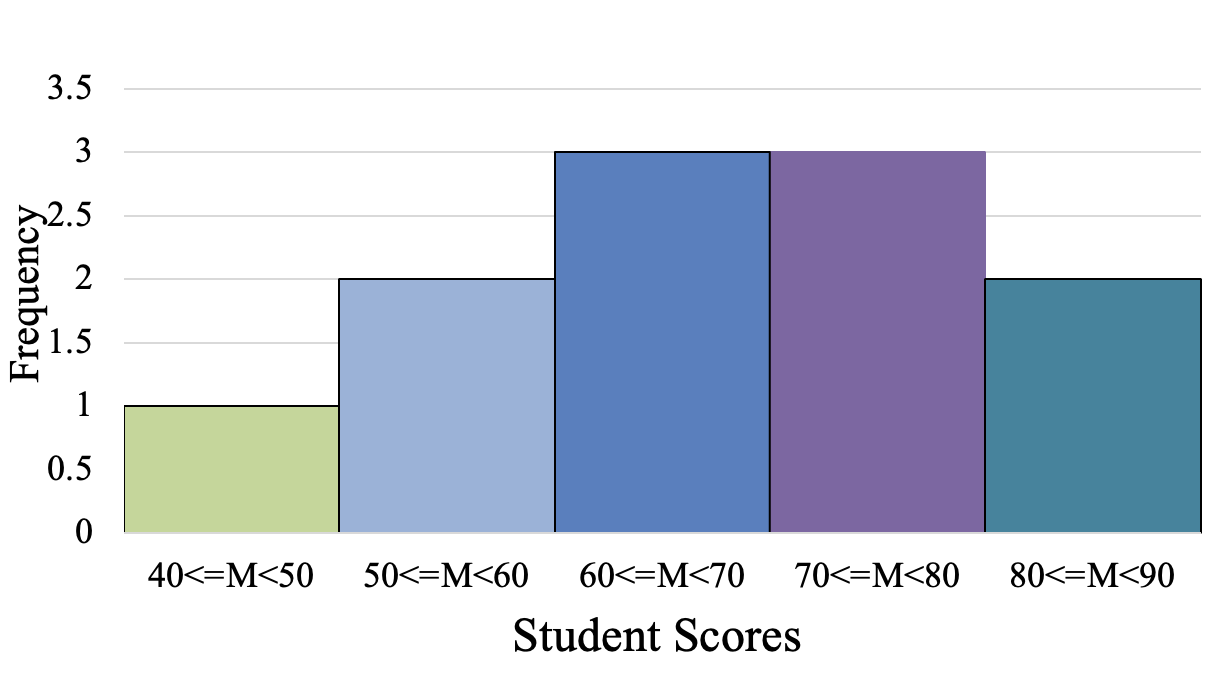
\includegraphics{Fig/q5_histogram.png}

}

\end{figure}
\end{frame}

\begin{frame}{Exercise 5 (Cont'd)}
\protect\hypertarget{exercise-5-contd}{}
\textbf{A:} We can only guess what the data points in each bin are. For
instance, a data point located in the first bin \((40 \le M < 50)\) can
be \(40, 40.12, 45\), etc. A reasonable way is to assume that this data
point is in the middle of the first bin. Therefore, we assume the first
data point is 45. Using the same argument, we assume that the two data
points located in the second bin are equal to the middle of the second
bin (55). Thus, the data set can be assumed as follows:

\vspace{5pt}

\scriptsize
\begin{table}
\centering
\begin{tabular}{ccccccccccc}
1 & 2 & 3 & 4 & 5 & 6 & 7 & 8 & 9 & 10 & 11 \\[3pt]
45 & 55 & 55 & 65 & 65 & 65 & 75 & 75 & 75 & 85 & 85 \\
\end{tabular}
\end{table}
\normalsize

Hence,

\begin{itemize}
\item
  \(\text{Mean} = \frac{\sum_{i=1}^{n} X_i}{n} = \frac{45 + 55 + \cdots + 85 + 85}{11} = \frac{745}{11} = 67.727\)
\item
  \(\text{Median} = X_{\frac{11+1}{2}} = X_6 = 65\)
\item
  \(\text{Mode: } 65 \text{ and } 75\)
\end{itemize}
\end{frame}

\begin{frame}{Exercise 5 (Cont'd)}
\protect\hypertarget{exercise-5-contd-1}{}
\begin{itemize}
\item
  Variance: \[
    \begin{aligned}
    S^2 & = \frac{\sum_{i=1}^{n}(X_i - \bar{X})^2}{n - 1} \\
                       &= \frac{(45 - 67.72)^2 + (55 - 67.72)^2 + \cdots + (85 - 67.72)^2}{11 - 1}  \\ 
                       &= \frac{1618.18}{10} = 161.81
    \end{aligned}
    \]
\item
  \(\text{Standard Deviation: } S = \sqrt{161.81} = 12.720\)
\end{itemize}
\end{frame}



\end{document}
